%==========================================================================
% Data Mining -- Lab 3: Decision Tree Analysis
%==========================================================================
\documentclass[12pt,a4paper]{article}

% -- Packages --------------------------------------------------------------
\usepackage[margin=2.5cm]{geometry}
\usepackage{graphicx}
\usepackage{booktabs}
\usepackage{array}
\usepackage{multirow}
\usepackage{caption}
\usepackage{subcaption}
\usepackage{float}
\usepackage{amsmath}
\usepackage{hyperref}
\usepackage{xcolor}
\usepackage{titlesec}
\usepackage{parskip}
\usepackage{fancyhdr}
\usepackage{enumitem}
\usepackage{lmodern}
\usepackage[T1]{fontenc}

% -- Colours & formatting --------------------------------------------------
\definecolor{myblue}{RGB}{30,100,170}
\hypersetup{colorlinks=true, linkcolor=myblue, urlcolor=myblue, citecolor=myblue}
\titleformat{\section}{\large\bfseries\color{myblue}}{\thesection}{1em}{}
\titleformat{\subsection}{\normalsize\bfseries\color{myblue}}{\thesubsection}{1em}{}
\titleformat{\subsubsection}{\normalsize\itshape\color{myblue}}{\thesubsubsection}{1em}{}

% -- Header / Footer -------------------------------------------------------
\pagestyle{fancy}
\fancyhf{}
\rhead{\small Data Mining -- Lab 3}
\lhead{\small Decision Tree Analysis}
\rfoot{\small\thepage}
\renewcommand{\headrulewidth}{0.4pt}

%==========================================================================
\begin{document}

%==========================================================================
% Cover Page
%==========================================================================
\begin{titlepage}
\centering
\vspace*{2cm}

{\Huge\bfseries\color{myblue} Data Mining}\\[0.4cm]
{\LARGE\bfseries Laboratory Report --- Lab 3}\\[0.3cm]
\rule{\linewidth}{0.5pt}\\[0.5cm]
{\Large Decision Tree Classification}\\[0.2cm]
{\large Gini vs.\ Entropy $\mid$ Holdout \& Cross-Validation $\mid$ Depth Analysis}\\[0.5cm]
\rule{\linewidth}{0.5pt}

\vspace{1.5cm}

{\large\bfseries Group Members}\\[0.5cm]
\begin{tabular}{@{}ll@{}}
\toprule
\textbf{Name} & \textbf{Student ID} \\
\midrule
Abdullah & --- \\
Member 2 & --- \\
Member 3 & --- \\
\bottomrule
\end{tabular}

\vspace{1.5cm}

{\large\bfseries Course Information}\\[0.5cm]
\begin{tabular}{@{}ll@{}}
Course     & Data Mining \\
Lab Number & 3 \\
Date       & \today \\
\end{tabular}

\vspace{2cm}

\textbf{Datasets:}\\[0.3cm]
\begin{tabular}{@{}ll@{}}
\textit{German Credit}  & 1000 instances, 24 numeric features, 2 classes \\
\textit{Waveform v1}    & 5000 instances, 21 continuous features, 3 classes \\
\end{tabular}

\vfill
{\small Department of Computer Science}
\end{titlepage}

%==========================================================================
\tableofcontents
\newpage

%==========================================================================
\section{Introduction}
%==========================================================================

Decision Trees are one of the most interpretable supervised learning
algorithms. They recursively partition the feature space by selecting the
split that maximises an impurity criterion, producing a flowchart-like
model that can be directly inspected.

This report evaluates decision tree classifiers on two benchmark datasets
from the UCI Machine Learning Repository:

\begin{itemize}
  \item \textbf{German Credit} (1\,000 samples, 24 numeric features,
    binary label: 0 = good credit, 1 = bad credit; 70\,\%/30\,\% split).
  \item \textbf{Waveform} (5\,000 samples, 21 continuous features,
    3-class label: 0, 1, 2; balanced classes, each $\approx 33\%$).
\end{itemize}

Three evaluation protocols are studied:

\begin{description}[style=nextline]
  \item[Part I --- Gini impurity.]
    Holdout (90/10 split, 5 repeated trials) and 10-fold cross-validation.
  \item[Part II --- Entropy impurity.]
    Same evaluation protocol; results compared with Part I.
  \item[Part III --- Tree depth.]
    Effect of \texttt{max\_depth} on training and test accuracy using the
    holdout method.
\end{description}

All experiments use \texttt{scikit-learn}. Precision and F-measure are
computed with \emph{weighted} averaging to correctly handle class imbalance.

%==========================================================================
\section{Part I --- Decision Tree with Gini Impurity}
%==========================================================================

\subsection{German Credit Dataset}

\subsubsection{Holdout Method (90/10, 5 Trials)}

The dataset is split 90\,\% training / 10\,\% test using a different
random seed for each trial. A full-depth
\texttt{DecisionTreeClassifier(criterion=`gini')} is trained and
evaluated on the held-out 10\,\% each time.

\begin{table}[H]
\centering
\caption{German Credit --- Holdout Results (Gini)}
\label{tab:ger_ho_gini}
\begin{tabular}{@{}lccc@{}}
\toprule
\textbf{Trial} & \textbf{Accuracy} & \textbf{Precision} & \textbf{F-measure} \\
\midrule
Trial 1  & 0.6600 & 0.7044 & 0.6762 \\
Trial 2  & 0.6700 & 0.6669 & 0.6684 \\
Trial 3  & 0.6600 & 0.6491 & 0.6535 \\
Trial 4  & 0.6500 & 0.6471 & 0.6485 \\
Trial 5  & 0.6300 & 0.6499 & 0.6385 \\
\midrule
\textbf{Average} & \textbf{0.6540} & \textbf{0.6635} & \textbf{0.6570} \\
\bottomrule
\end{tabular}
\end{table}

\begin{figure}[H]
\centering
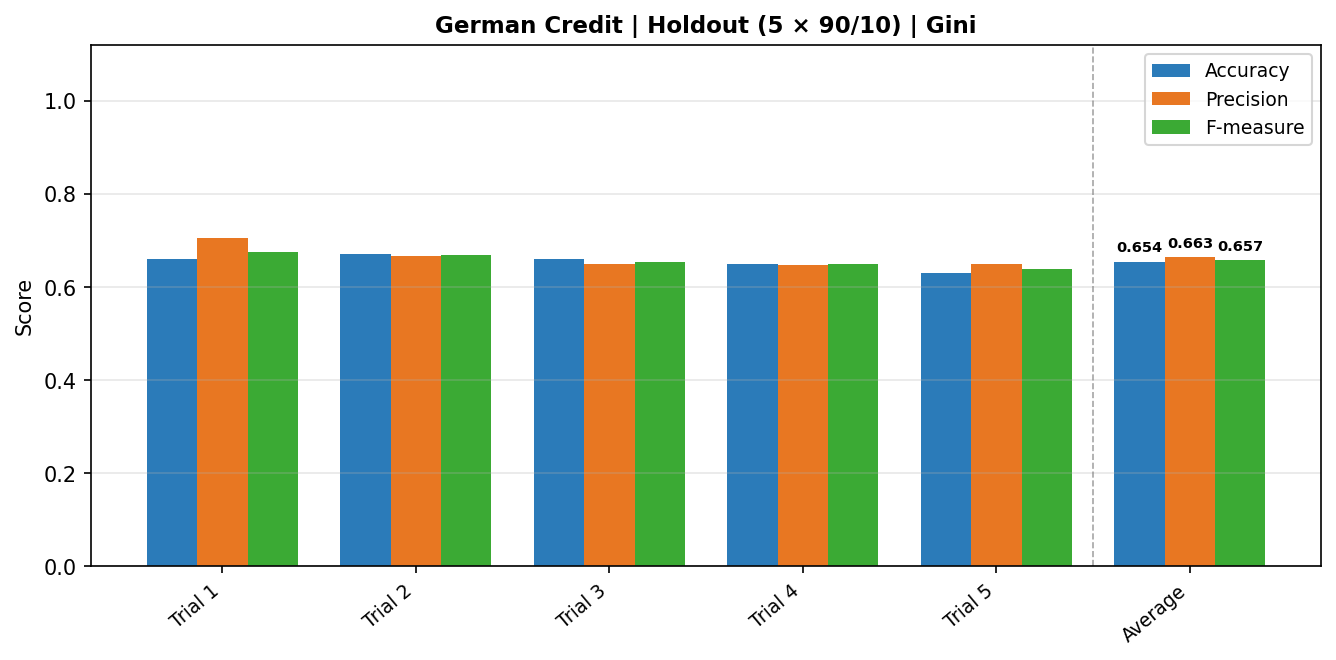
\includegraphics[width=0.95\linewidth]{output/german_holdout_gini.png}
\caption{German Credit --- Holdout metrics per trial (Gini)}
\label{fig:ger_ho_gini}
\end{figure}

\subsubsection{10-Fold Cross-Validation}

\begin{table}[H]
\centering
\caption{German Credit --- 10-Fold CV Results (Gini)}
\label{tab:ger_cv_gini}
\begin{tabular}{@{}lccc@{}}
\toprule
\textbf{Fold} & \textbf{Accuracy} & \textbf{Precision} & \textbf{F-measure} \\
\midrule
Fold 1   & 0.6600 & 0.7044 & 0.6762 \\
Fold 2   & 0.6300 & 0.6329 & 0.6314 \\
Fold 3   & 0.7000 & 0.6936 & 0.6965 \\
Fold 4   & 0.7300 & 0.7454 & 0.7342 \\
Fold 5   & 0.7200 & 0.7141 & 0.7167 \\
Fold 6   & 0.5900 & 0.6300 & 0.6058 \\
Fold 7   & 0.7300 & 0.7215 & 0.7238 \\
Fold 8   & 0.6700 & 0.6894 & 0.6781 \\
Fold 9   & 0.6500 & 0.6832 & 0.6617 \\
Fold 10  & 0.7200 & 0.7163 & 0.7178 \\
\midrule
\textbf{Average} & \textbf{0.6800} & \textbf{0.6931} & \textbf{0.6842} \\
\bottomrule
\end{tabular}
\end{table}

\begin{figure}[H]
\centering
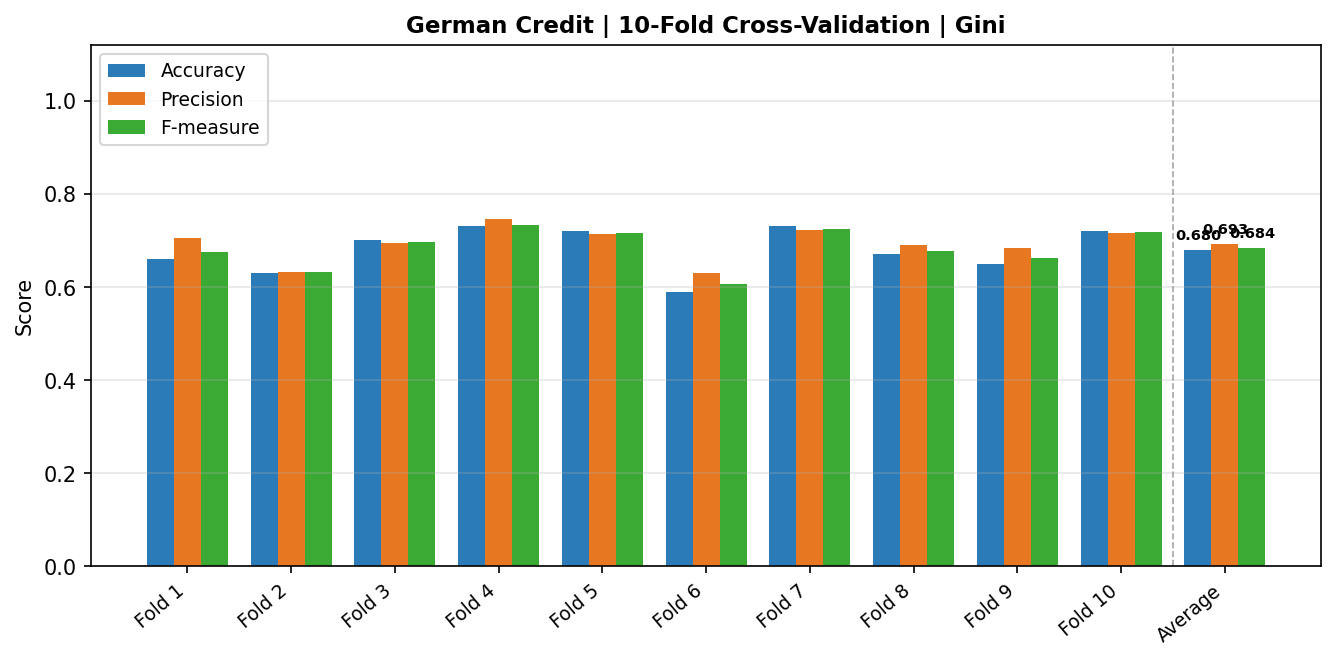
\includegraphics[width=0.95\linewidth]{output/german_cv_gini.png}
\caption{German Credit --- 10-Fold CV metrics per fold (Gini)}
\label{fig:ger_cv_gini}
\end{figure}

%-------------------------------------------------------------------------
\subsection{Waveform Dataset}

\subsubsection{Holdout Method (90/10, 5 Trials)}

\begin{table}[H]
\centering
\caption{Waveform --- Holdout Results (Gini)}
\label{tab:wav_ho_gini}
\begin{tabular}{@{}lccc@{}}
\toprule
\textbf{Trial} & \textbf{Accuracy} & \textbf{Precision} & \textbf{F-measure} \\
\midrule
Trial 1  & 0.7440 & 0.7467 & 0.7438 \\
Trial 2  & 0.7160 & 0.7180 & 0.7162 \\
Trial 3  & 0.7760 & 0.7781 & 0.7763 \\
Trial 4  & 0.7400 & 0.7405 & 0.7394 \\
Trial 5  & 0.7680 & 0.7680 & 0.7679 \\
\midrule
\textbf{Average} & \textbf{0.7488} & \textbf{0.7503} & \textbf{0.7487} \\
\bottomrule
\end{tabular}
\end{table}

\begin{figure}[H]
\centering
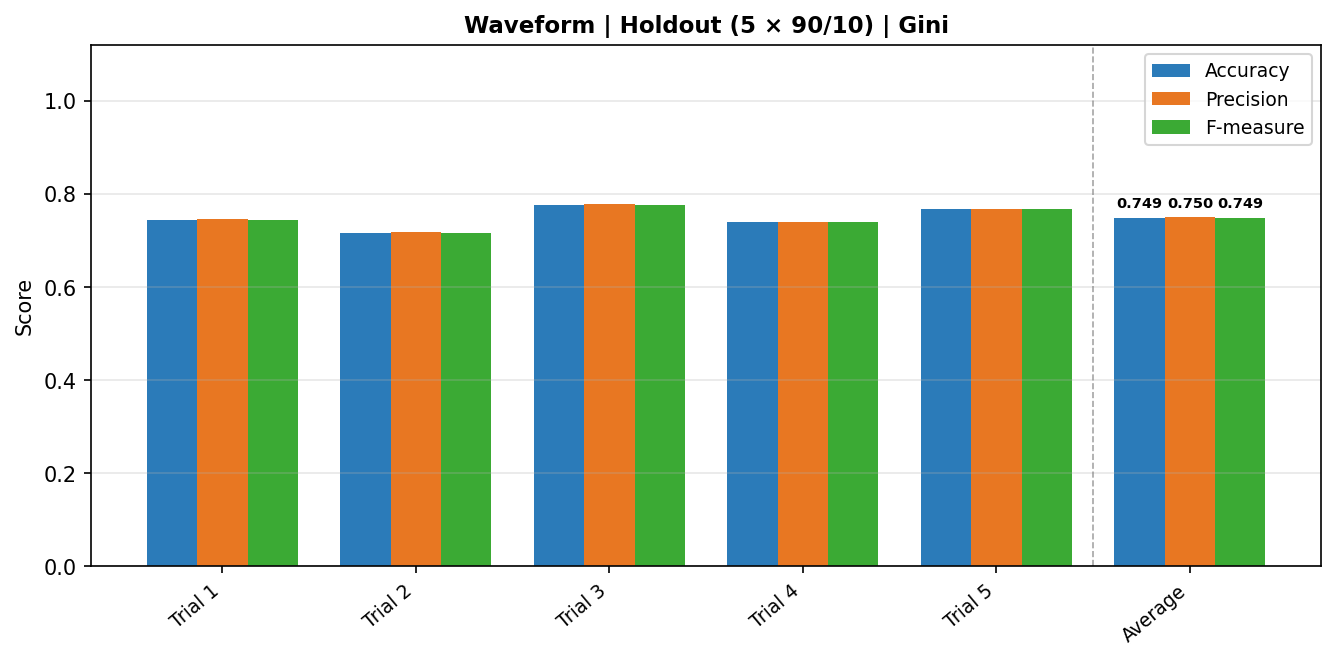
\includegraphics[width=0.95\linewidth]{output/wave_holdout_gini.png}
\caption{Waveform --- Holdout metrics per trial (Gini)}
\label{fig:wav_ho_gini}
\end{figure}

\subsubsection{10-Fold Cross-Validation}

\begin{table}[H]
\centering
\caption{Waveform --- 10-Fold CV Results (Gini)}
\label{tab:wav_cv_gini}
\begin{tabular}{@{}lccc@{}}
\toprule
\textbf{Fold} & \textbf{Accuracy} & \textbf{Precision} & \textbf{F-measure} \\
\midrule
Fold 1   & 0.7440 & 0.7467 & 0.7438 \\
Fold 2   & 0.7440 & 0.7444 & 0.7437 \\
Fold 3   & 0.7680 & 0.7698 & 0.7682 \\
Fold 4   & 0.7440 & 0.7448 & 0.7441 \\
Fold 5   & 0.7340 & 0.7362 & 0.7344 \\
Fold 6   & 0.7560 & 0.7555 & 0.7552 \\
Fold 7   & 0.7720 & 0.7729 & 0.7713 \\
Fold 8   & 0.7700 & 0.7704 & 0.7700 \\
Fold 9   & 0.7180 & 0.7189 & 0.7179 \\
Fold 10  & 0.7080 & 0.7101 & 0.7085 \\
\midrule
\textbf{Average} & \textbf{0.7458} & \textbf{0.7470} & \textbf{0.7457} \\
\bottomrule
\end{tabular}
\end{table}

\begin{figure}[H]
\centering
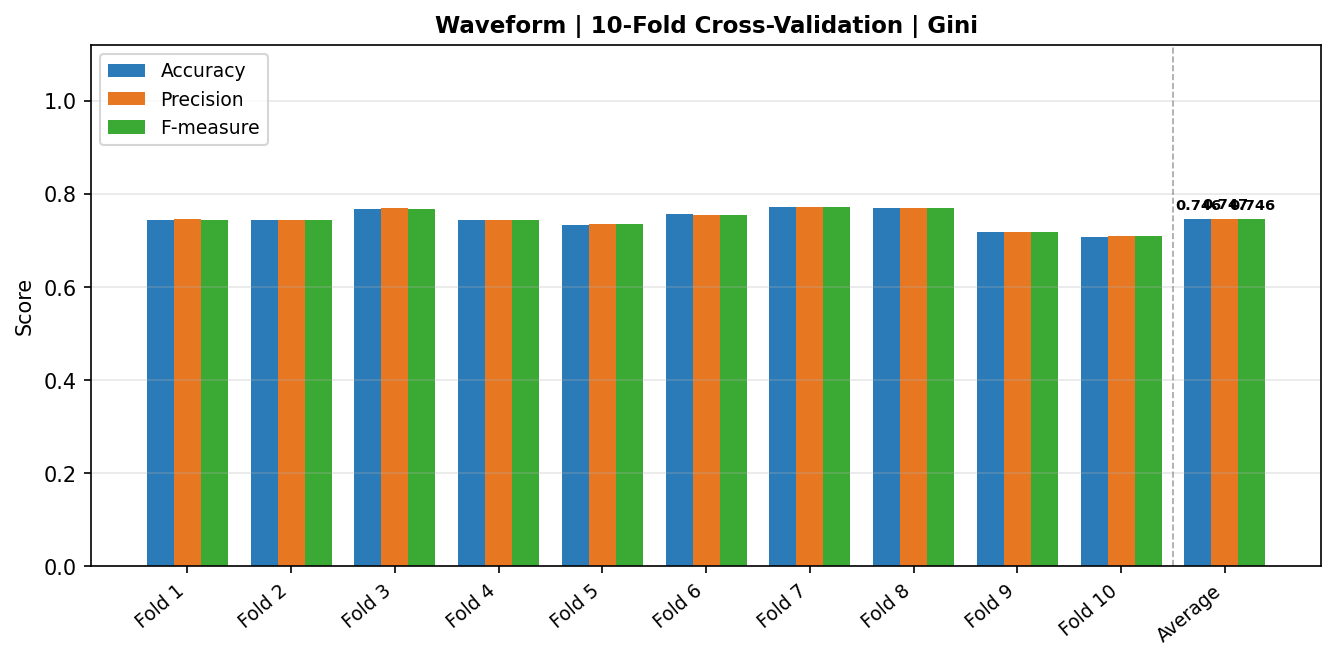
\includegraphics[width=0.95\linewidth]{output/wave_cv_gini.png}
\caption{Waveform --- 10-Fold CV metrics per fold (Gini)}
\label{fig:wav_cv_gini}
\end{figure}

%==========================================================================
\section{Part II --- Decision Tree with Entropy Impurity}
%==========================================================================

\subsection{German Credit Dataset}

\subsubsection{Holdout Method (90/10, 5 Trials)}

\begin{table}[H]
\centering
\caption{German Credit --- Holdout Results (Entropy)}
\label{tab:ger_ho_ent}
\begin{tabular}{@{}lccc@{}}
\toprule
\textbf{Trial} & \textbf{Accuracy} & \textbf{Precision} & \textbf{F-measure} \\
\midrule
Trial 1  & 0.7000 & 0.7329 & 0.7122 \\
Trial 2  & 0.6400 & 0.6609 & 0.6483 \\
Trial 3  & 0.6500 & 0.6716 & 0.6578 \\
Trial 4  & 0.6800 & 0.6749 & 0.6772 \\
Trial 5  & 0.6600 & 0.6600 & 0.6600 \\
\midrule
\textbf{Average} & \textbf{0.6660} & \textbf{0.6801} & \textbf{0.6711} \\
\bottomrule
\end{tabular}
\end{table}

\begin{figure}[H]
\centering
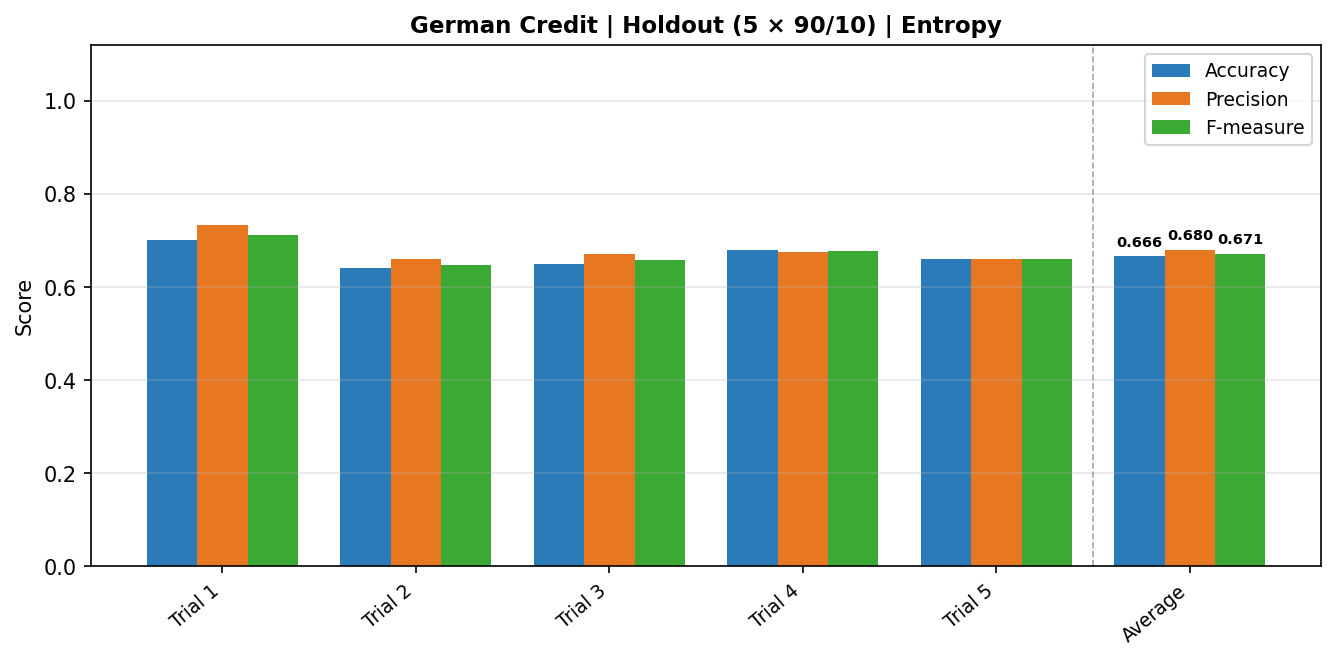
\includegraphics[width=0.95\linewidth]{output/german_holdout_entropy.png}
\caption{German Credit --- Holdout metrics per trial (Entropy)}
\label{fig:ger_ho_ent}
\end{figure}

\subsubsection{10-Fold Cross-Validation}

\begin{table}[H]
\centering
\caption{German Credit --- 10-Fold CV Results (Entropy)}
\label{tab:ger_cv_ent}
\begin{tabular}{@{}lccc@{}}
\toprule
\textbf{Fold} & \textbf{Accuracy} & \textbf{Precision} & \textbf{F-measure} \\
\midrule
Fold 1   & 0.7000 & 0.7329 & 0.7122 \\
Fold 2   & 0.6400 & 0.6400 & 0.6400 \\
Fold 3   & 0.7700 & 0.7632 & 0.7658 \\
Fold 4   & 0.7500 & 0.7486 & 0.7492 \\
Fold 5   & 0.7500 & 0.7342 & 0.7379 \\
Fold 6   & 0.6200 & 0.6626 & 0.6357 \\
Fold 7   & 0.6900 & 0.6877 & 0.6888 \\
Fold 8   & 0.6200 & 0.6626 & 0.6357 \\
Fold 9   & 0.6900 & 0.6869 & 0.6884 \\
Fold 10  & 0.7000 & 0.6924 & 0.6950 \\
\midrule
\textbf{Average} & \textbf{0.6930} & \textbf{0.7011} & \textbf{0.6949} \\
\bottomrule
\end{tabular}
\end{table}

\begin{figure}[H]
\centering
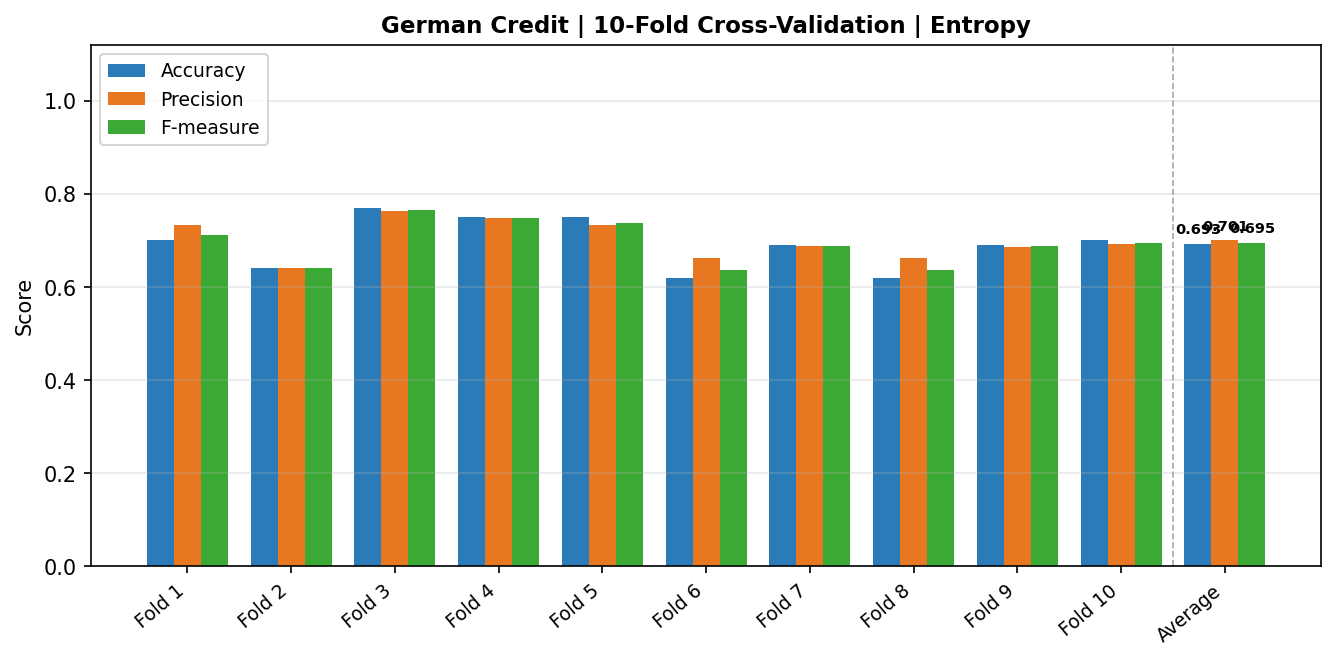
\includegraphics[width=0.95\linewidth]{output/german_cv_entropy.png}
\caption{German Credit --- 10-Fold CV metrics per fold (Entropy)}
\label{fig:ger_cv_ent}
\end{figure}

%-------------------------------------------------------------------------
\subsection{Waveform Dataset}

\subsubsection{Holdout Method (90/10, 5 Trials)}

\begin{table}[H]
\centering
\caption{Waveform --- Holdout Results (Entropy)}
\label{tab:wav_ho_ent}
\begin{tabular}{@{}lccc@{}}
\toprule
\textbf{Trial} & \textbf{Accuracy} & \textbf{Precision} & \textbf{F-measure} \\
\midrule
Trial 1  & 0.7360 & 0.7392 & 0.7359 \\
Trial 2  & 0.7440 & 0.7468 & 0.7445 \\
Trial 3  & 0.7320 & 0.7363 & 0.7330 \\
Trial 4  & 0.7920 & 0.7919 & 0.7919 \\
Trial 5  & 0.7400 & 0.7409 & 0.7401 \\
\midrule
\textbf{Average} & \textbf{0.7488} & \textbf{0.7510} & \textbf{0.7491} \\
\bottomrule
\end{tabular}
\end{table}

\begin{figure}[H]
\centering
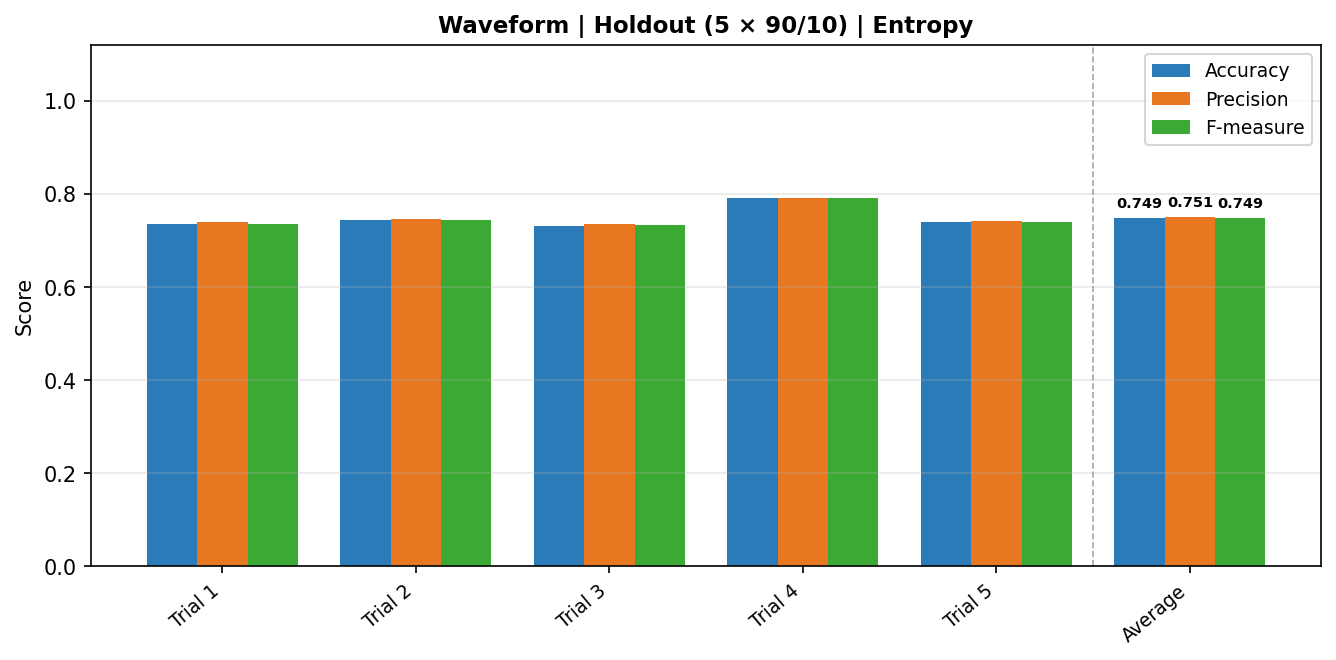
\includegraphics[width=0.95\linewidth]{output/wave_holdout_entropy.png}
\caption{Waveform --- Holdout metrics per trial (Entropy)}
\label{fig:wav_ho_ent}
\end{figure}

\subsubsection{10-Fold Cross-Validation}

\begin{table}[H]
\centering
\caption{Waveform --- 10-Fold CV Results (Entropy)}
\label{tab:wav_cv_ent}
\begin{tabular}{@{}lccc@{}}
\toprule
\textbf{Fold} & \textbf{Accuracy} & \textbf{Precision} & \textbf{F-measure} \\
\midrule
Fold 1   & 0.7360 & 0.7392 & 0.7359 \\
Fold 2   & 0.7780 & 0.7778 & 0.7775 \\
Fold 3   & 0.7460 & 0.7488 & 0.7469 \\
Fold 4   & 0.7520 & 0.7513 & 0.7514 \\
Fold 5   & 0.7680 & 0.7681 & 0.7680 \\
Fold 6   & 0.7640 & 0.7640 & 0.7637 \\
Fold 7   & 0.7540 & 0.7537 & 0.7537 \\
Fold 8   & 0.7520 & 0.7520 & 0.7520 \\
Fold 9   & 0.7720 & 0.7717 & 0.7717 \\
Fold 10  & 0.7580 & 0.7591 & 0.7578 \\
\midrule
\textbf{Average} & \textbf{0.7580} & \textbf{0.7586} & \textbf{0.7579} \\
\bottomrule
\end{tabular}
\end{table}

\begin{figure}[H]
\centering
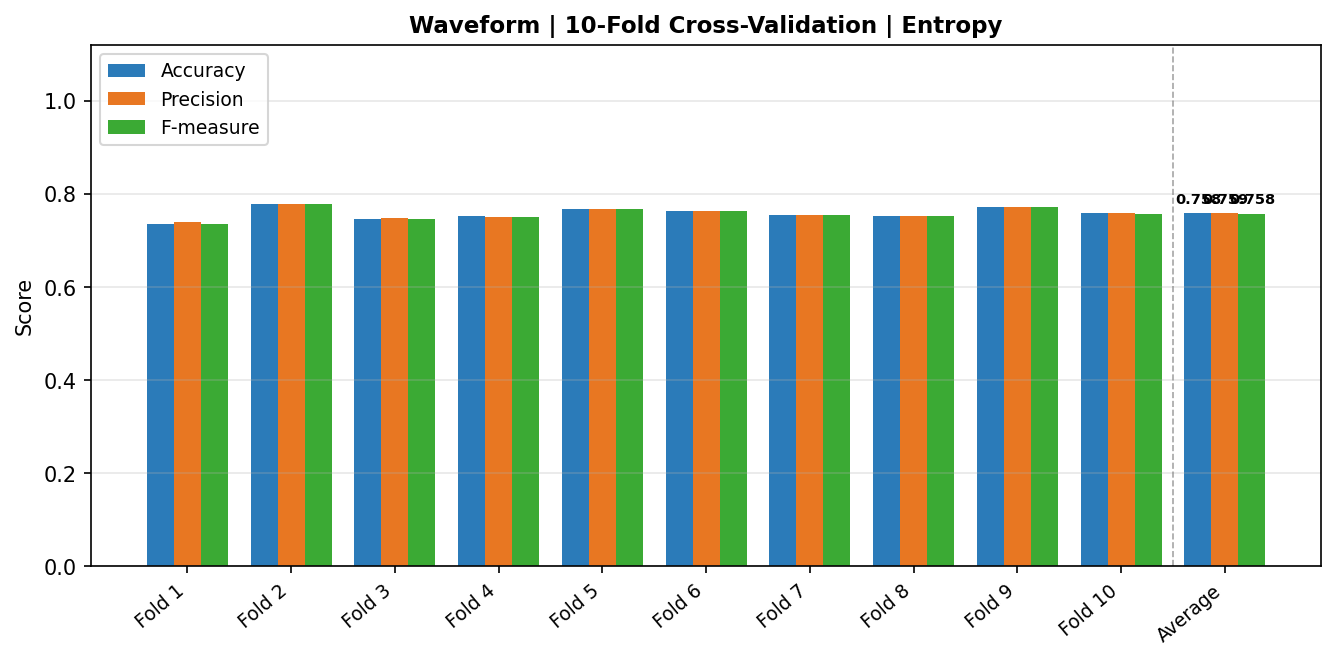
\includegraphics[width=0.95\linewidth]{output/wave_cv_entropy.png}
\caption{Waveform --- 10-Fold CV metrics per fold (Entropy)}
\label{fig:wav_cv_ent}
\end{figure}

%-------------------------------------------------------------------------
\subsection{Comparison: Gini vs.\ Entropy (CV Accuracy)}

Table~\ref{tab:compare_cv} summarises the average 10-fold CV accuracy for
both impurity measures across both datasets.

\begin{table}[H]
\centering
\caption{Average 10-Fold CV Accuracy --- Gini vs.\ Entropy}
\label{tab:compare_cv}
\begin{tabular}{@{}lcc@{}}
\toprule
\textbf{Dataset} & \textbf{Gini} & \textbf{Entropy} \\
\midrule
German Credit & 0.6800 & 0.6930 \\
Waveform      & 0.7458 & 0.7580 \\
\bottomrule
\end{tabular}
\end{table}

Figures~\ref{fig:ger_compare} and~\ref{fig:wav_compare} show the
fold-by-fold accuracy and an aggregate bar comparison.

\begin{figure}[H]
\centering
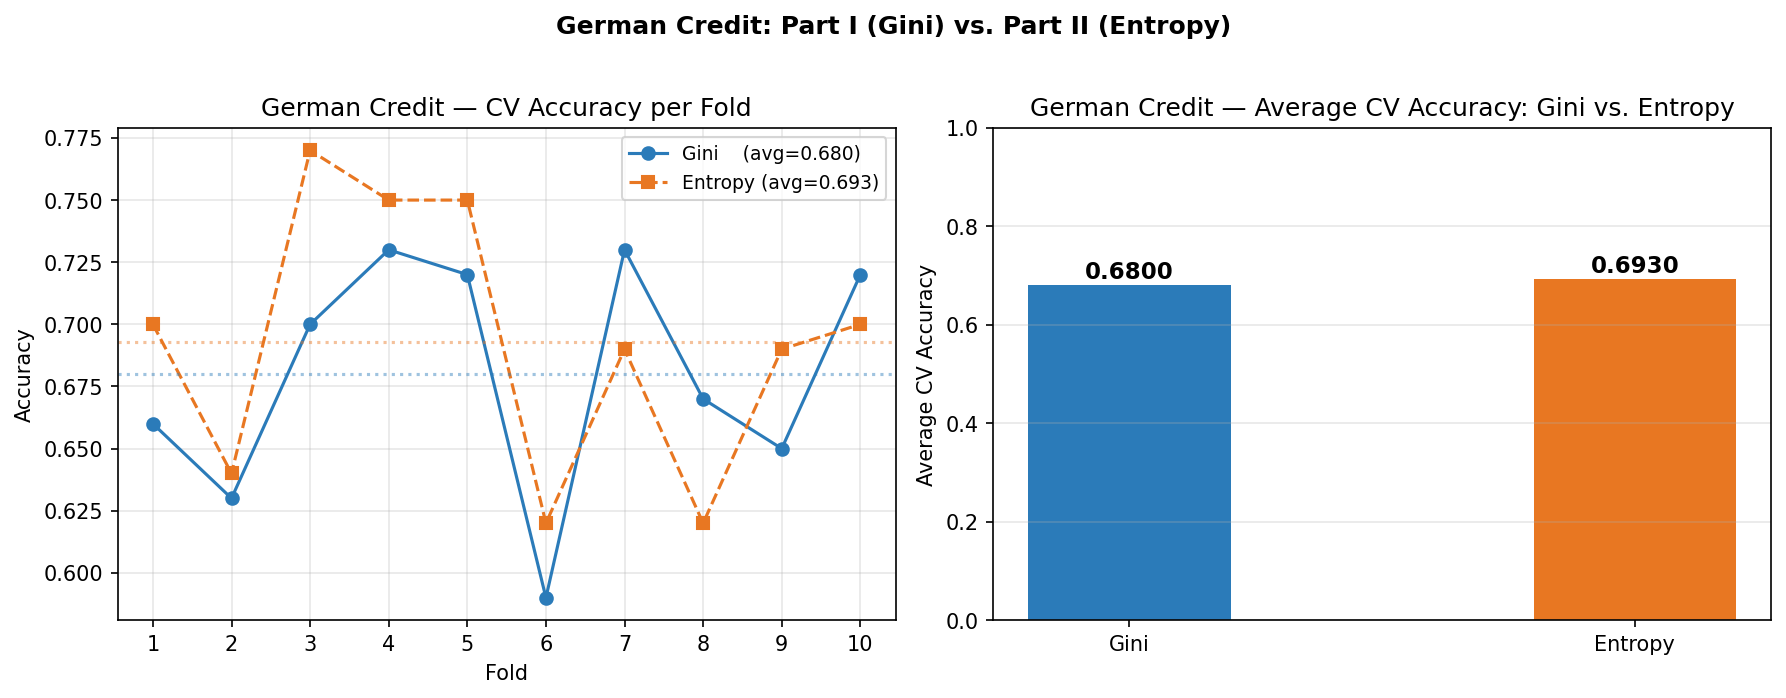
\includegraphics[width=0.97\linewidth]{output/german_compare_cv.png}
\caption{German Credit --- CV accuracy per fold: Gini vs.\ Entropy (left)
  and average comparison bar chart (right).}
\label{fig:ger_compare}
\end{figure}

\begin{figure}[H]
\centering
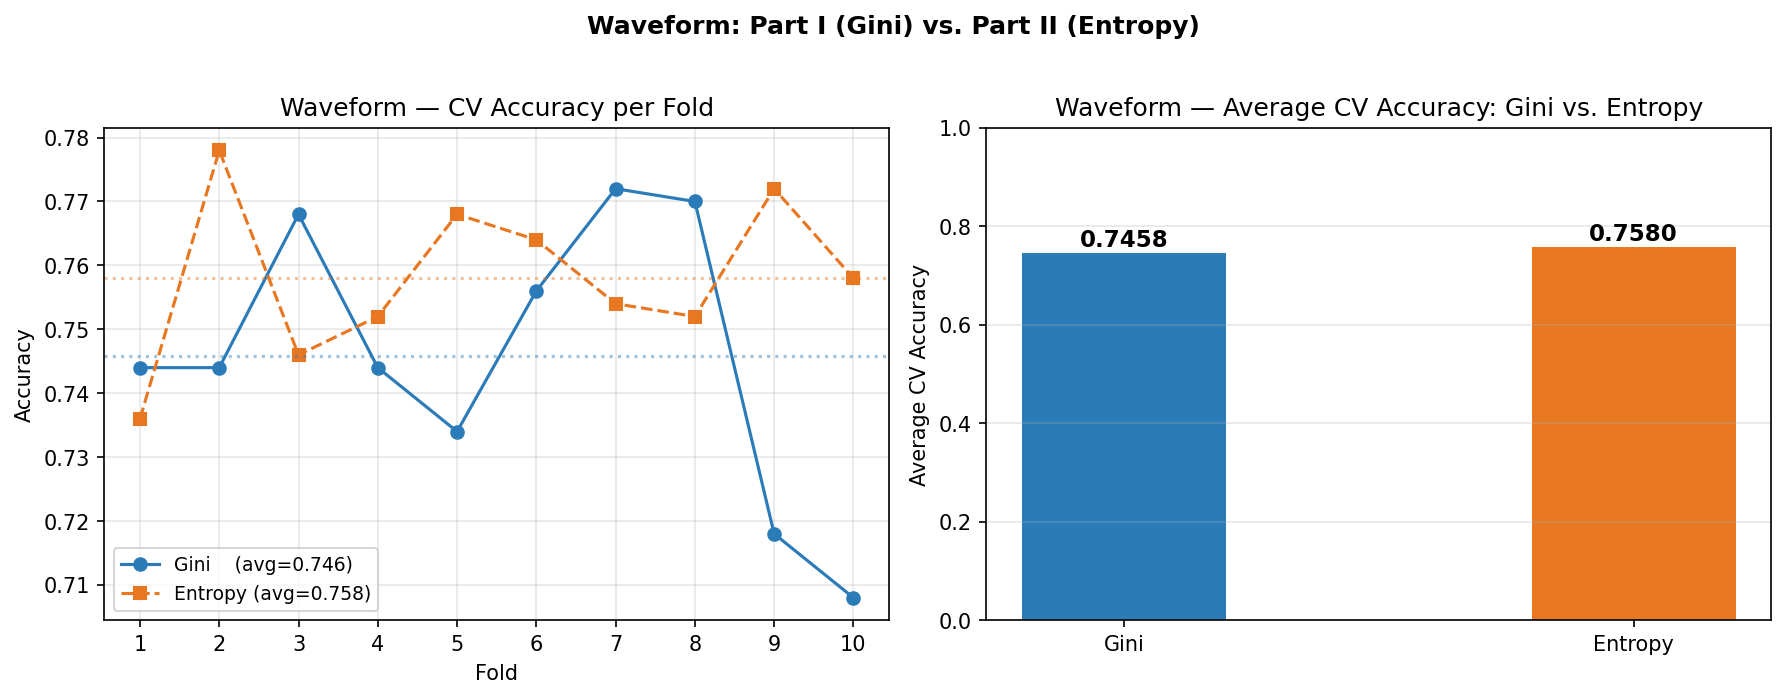
\includegraphics[width=0.97\linewidth]{output/wave_compare_cv.png}
\caption{Waveform --- CV accuracy per fold: Gini vs.\ Entropy (left)
  and average comparison bar chart (right).}
\label{fig:wav_compare}
\end{figure}

\subsubsection{Discussion}

Entropy achieves marginally higher average CV accuracy on both datasets:

\begin{itemize}
  \item \textbf{German Credit}: Gini $= 0.680$, Entropy $= 0.693$
    (difference $= +0.013$).
  \item \textbf{Waveform}: Gini $= 0.746$, Entropy $= 0.758$
    (difference $= +0.012$).
\end{itemize}

The differences are small, consistent with empirical literature showing
that Gini and Information Gain (Entropy) select the same split in the
vast majority of cases~\cite{Breiman1984}. Entropy is slightly more
expensive computationally (requires a logarithm) but the cost is
negligible at these dataset sizes. The marginal improvement of Entropy
may be attributed to its tendency to create more balanced splits, which
can help on class-imbalanced tasks such as German Credit.

%==========================================================================
\section{Part III --- Effect of Tree Depth on Accuracy}
%==========================================================================

\subsection{Setup}

Using a single 90/10 holdout split with \texttt{criterion=`gini'}, the
\texttt{max\_depth} parameter is varied over
$\{2,\,5,\,8,\,11,\,14,\,17,\,20,\,23,\,26,\,29,\,32,\,35,\,38,\,41,\,44,\,47,\,50\}$.
For each depth, both training accuracy (on the 90\,\% partition) and
test accuracy (on the 10\,\% partition) are recorded.

\subsection{German Credit}

\begin{table}[H]
\centering
\caption{German Credit --- Training \& Test Accuracy vs.\ Max Depth (Gini)}
\label{tab:ger_depth}
\begin{tabular}{@{}rcc@{}}
\toprule
\textbf{Max Depth} & \textbf{Train Accuracy} & \textbf{Test Accuracy} \\
\midrule
 2 & 0.7311 & 0.7300 \\
 5 & 0.8067 & \textbf{0.7400} \\
 8 & 0.9100 & 0.6900 \\
11 & 0.9689 & 0.6700 \\
14 & 0.9944 & 0.6300 \\
17 & 1.0000 & 0.6600 \\
20 & 1.0000 & 0.6600 \\
23 & 1.0000 & 0.6600 \\
26 & 1.0000 & 0.6600 \\
29 & 1.0000 & 0.6600 \\
32 & 1.0000 & 0.6600 \\
35 & 1.0000 & 0.6600 \\
38 & 1.0000 & 0.6600 \\
41 & 1.0000 & 0.6600 \\
44 & 1.0000 & 0.6600 \\
47 & 1.0000 & 0.6600 \\
50 & 1.0000 & 0.6600 \\
\bottomrule
\end{tabular}
\end{table}

\begin{figure}[H]
\centering
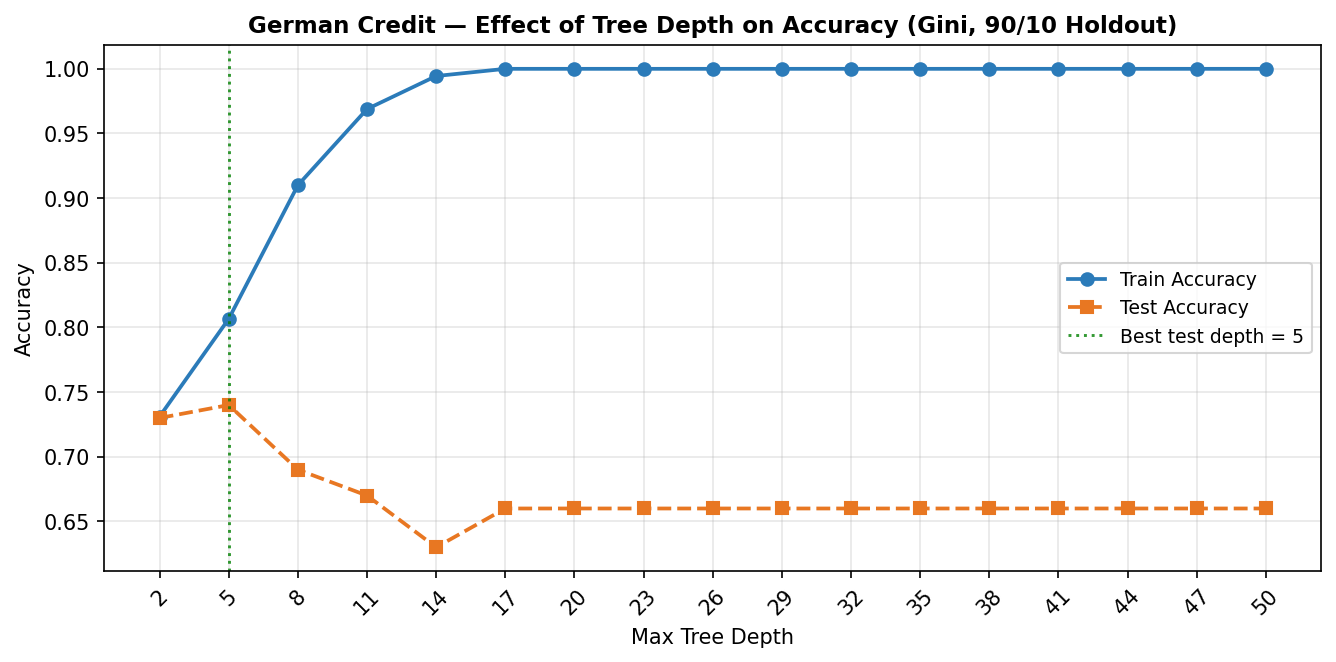
\includegraphics[width=0.95\linewidth]{output/german_depth_effect.png}
\caption{German Credit --- Training vs.\ Test Accuracy as a function of
  Max Tree Depth (Gini, single 90/10 holdout).}
\label{fig:ger_depth}
\end{figure}

\subsection{Waveform}

\begin{table}[H]
\centering
\caption{Waveform --- Training \& Test Accuracy vs.\ Max Depth (Gini)}
\label{tab:wav_depth}
\begin{tabular}{@{}rcc@{}}
\toprule
\textbf{Max Depth} & \textbf{Train Accuracy} & \textbf{Test Accuracy} \\
\midrule
 2 & 0.7031 & 0.7180 \\
 5 & 0.7996 & 0.7700 \\
 8 & 0.9084 & \textbf{0.7940} \\
11 & 0.9678 & 0.7720 \\
14 & 0.9918 & 0.7800 \\
17 & 0.9993 & 0.7480 \\
20 & 1.0000 & 0.7440 \\
23 & 1.0000 & 0.7440 \\
26 & 1.0000 & 0.7440 \\
29 & 1.0000 & 0.7440 \\
32 & 1.0000 & 0.7440 \\
35 & 1.0000 & 0.7440 \\
38 & 1.0000 & 0.7440 \\
41 & 1.0000 & 0.7440 \\
44 & 1.0000 & 0.7440 \\
47 & 1.0000 & 0.7440 \\
50 & 1.0000 & 0.7440 \\
\bottomrule
\end{tabular}
\end{table}

\begin{figure}[H]
\centering
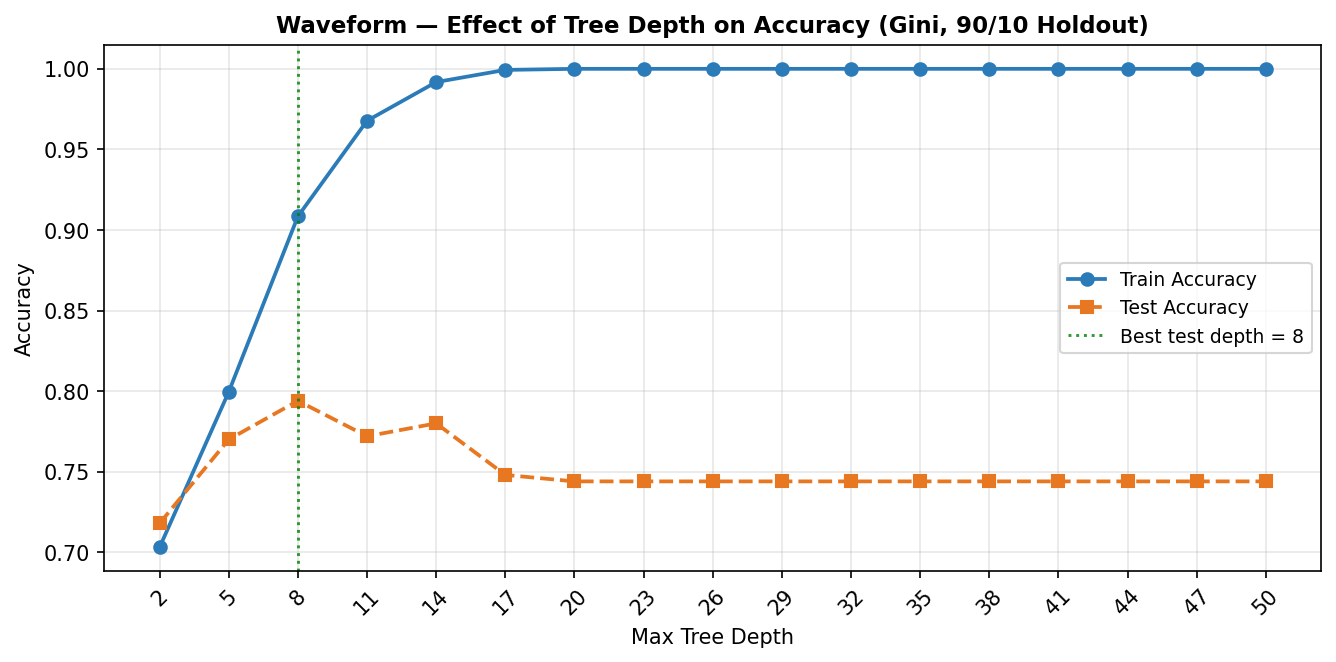
\includegraphics[width=0.95\linewidth]{output/wave_depth_effect.png}
\caption{Waveform --- Training vs.\ Test Accuracy as a function of
  Max Tree Depth (Gini, single 90/10 holdout).}
\label{fig:wav_depth}
\end{figure}

\subsection{Observations and Discussion}

The depth plots reveal a textbook \textbf{bias--variance trade-off}:

\paragraph{Training accuracy} increases monotonically with depth in both
datasets, reaching 100\,\% once the tree is deep enough to perfectly
memorise the training set. For German Credit, saturation occurs around
depth~17; for Waveform, around depth~20.

\paragraph{Test accuracy --- German Credit.}
Test accuracy peaks early (\textbf{depth = 5}, test accuracy = 0.740)
and then \emph{decreases} as the tree grows deeper, stabilising at
0.660 for depths $\geq 17$. This is a clear sign of overfitting: the
increasingly complex tree fits training noise and fails to generalise.
The optimal depth lies in the range $[2,\,5]$.

\paragraph{Test accuracy --- Waveform.}
Test accuracy also peaks early (\textbf{depth = 8}, test accuracy = 0.794),
then declines and stabilises at 0.744 for depths $\geq 20$. The Waveform
task has more inherent complexity (three classes, additive noise), so a
slightly deeper tree is needed before the overfitting regime begins.

\paragraph{Key observation.}
There is a clear \emph{gap} between training and test accuracy that widens
as depth increases. Once the tree saturates to 100\,\% training accuracy,
the test accuracy is already well below its maximum, demonstrating the
danger of unconstrained tree growth.

\paragraph{Practical recommendation.}
These results strongly motivate \emph{pre-pruning} (limiting
\texttt{max\_depth}) or \emph{post-pruning} (cost-complexity pruning,
\texttt{ccp\_alpha} in scikit-learn). Ensemble methods such as Random
Forests mitigate this variance issue by averaging many shallow trees.

\begin{table}[H]
\centering
\caption{Summary: Best Test Accuracy and Corresponding Depth}
\label{tab:best_depth}
\begin{tabular}{@{}lccc@{}}
\toprule
\textbf{Dataset} & \textbf{Best Depth} & \textbf{Best Test Acc.}
  & \textbf{Saturated Test Acc.} \\
\midrule
German Credit & 5  & 0.740 & 0.660 \\
Waveform      & 8  & 0.794 & 0.744 \\
\bottomrule
\end{tabular}
\end{table}

%==========================================================================
\section{Summary and Conclusions}
%==========================================================================

\begin{itemize}
  \item \textbf{Holdout vs.\ Cross-Validation.}
    CV consistently yields higher and more stable accuracy estimates than a
    single holdout trial because all data points are used as test examples
    across folds. Variance between holdout trials (e.g., 0.630--0.700 for
    German Credit/Gini) illustrates the instability of a single 10\,\% test
    set at this sample size.

  \item \textbf{Gini vs.\ Entropy.}
    Entropy achieves marginally better accuracy ($+1$--$1.5$ percentage
    points) on both datasets. The computational overhead of Entropy is
    negligible at these scales, making it the preferred choice.

  \item \textbf{Tree Depth.}
    Full-depth trees overfit severely. Depth pruning at 5 (German Credit)
    and 8 (Waveform) recovers the best generalisation. Depths beyond
    17--20 add no test accuracy benefit on either dataset.

  \item \textbf{Dataset Characteristics.}
    The Waveform dataset (5\,000 samples, 3 balanced classes) supports
    higher accuracy ($\approx 75$--$80\,\%$) compared with German Credit
    ($\approx 65$--$74\,\%$), which has fewer samples, a harder decision
    boundary, and class imbalance (700:300).
\end{itemize}

%==========================================================================
\begin{thebibliography}{9}

\bibitem{Breiman1984}
  L.~Breiman, J.~Friedman, R.~Olshen, and C.~Stone,
  \textit{Classification and Regression Trees}.
  Wadsworth, Belmont, CA, 1984.

\bibitem{sklearn}
  F.~Pedregosa et~al.,
  ``Scikit-learn: Machine learning in Python,''
  \textit{Journal of Machine Learning Research}, vol.~12, pp.~2825--2830,
  2011.

\bibitem{uci_german}
  UCI Machine Learning Repository,
  \textit{Statlog (German Credit Data)}, 1994.

\bibitem{uci_waveform}
  UCI Machine Learning Repository,
  \textit{Waveform Database Generator (Version 1)}, 1988.

\end{thebibliography}

\end{document}
